The third prototype built, TRITIUM-Aveiro, is a proposal of the final TRITIUM detector module. This prototype, which is shown in Figure \ref{fig:TritiumAveiro0}, was designed and built in the workshop of the University of Aveiro. This prototype consists of a PTFE vessel (marked as D in Figure \ref{fig:TritiumAveiro0}), shown in Figure \ref{fig:TeflonStructureFibersTritiumAveiro0}, with an internal cylindrical hole of $43~\mm$ diameter and $18~\cm$ length.

\begin{figure}[h]
\centering
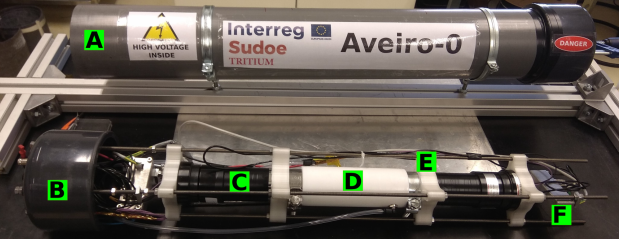
\includegraphics[scale=0.4]{5Prototypes/53FinalPrototypes/531TritiumAveiro/GeneralViewOfAveiroPrototype.png}
\caption{TRITIUM-Aveiro prototype.\label{fig:TritiumAveiro0}}
\end{figure}
 
\begin{figure}[h]
\centering
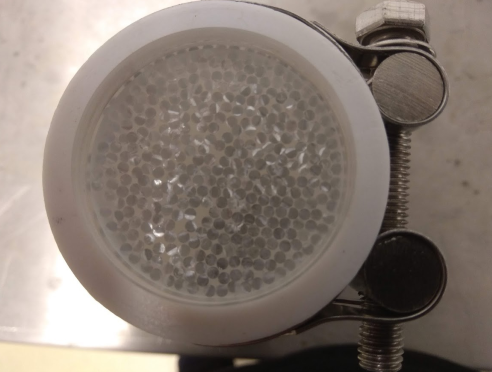
\includegraphics[scale=0.4]{5Prototypes/53FinalPrototypes/531TritiumAveiro/TeflonVessel_Fibers.png}
\caption{PTFE structure and fiber bundle used in TRITIUM-Aveiro prototype.\label{fig:TeflonStructureFibersTritiumAveiro0}}
\end{figure}
This vessel contains $360$ uncladded scintillating fibers of $180~\mm$ length. The fibers are BCF-10 from Saint-Gobain company \cite{DataSheetBCF10Fiber}, which have similar characteristics than the BCF-12 fibers, table \ref{tab:ParametersFibersBCF12}, except the diameter, which is $2~\mm$. In order to quantify the importance of the fiber diameter, the measurements are compared with similar measurements performed with the TRITIUM-IFIC-2 prototype, which has a similar configuration but with $1~\mm$ fibers.

The scintillator fibers are freely arranged within the PTFE vessel (without any PTFE matrix that fix them) and the number of fibers used is the maximum that allows water to flow around them. These fibers were cleaved with the device developed by TRITIUM, section \ref{subsubsec:CleavingProcess}, but they were neither polished nor cleaned because the automatic polishing machine was not yet developed and it was not feasible to polish 360 fibers by hand. 

The PTFE vessel is totally closed and  a water inlet/outlet were installed in it to allow a constant water flux through it. Two PMMA $10~\mm$ thick windows, located at both ends of the fiber bundle, are used to read out the fibers. Two clamps are used to make a tight junction of the PTFE walls and the PMMA. PMMA was chosen for its optical properties, especially its transmission coefficient, which is larger than $95\%$ at the scintillating fiber wavelength. Two PMTs (marked as C in Figure \ref{fig:TritiumAveiro0}) are used to read out this prototype in time coincidence, the HV of which was set at $-1500~\volt$. Its quantum efficiency is $26\%$. These PMTs are attached to both fiber bundle ends by two pieces (marked as E in Figure \ref{fig:TritiumAveiro0}) built with a 3D printer and they are optically coupled to the PMMA windows through optical grease \cite{OpticalGrease}. The PMTs used are R2154-02 2" from Hamamatsu \cite{DataSheetPMTsAveiro}, that have gain and efficiency quite similar to the PMTs used in the other TRITIUM prototypes.

This prototype and its electronics (marked as F in Figure \ref{fig:TritiumAveiro0}), were arranged in a structure, shown in Figure \ref{fig:TritiumAveiro0}, composed of several clamps and four stainless-steel screws, locked to an external PVC structure, marked as A and B in Figure \ref{fig:TritiumAveiro0}, which protects the prototype from physical damage and provides a light-tight operation environment. This PVC structure is equiped with the necessary feed-through connectors.

Only one prototype was built, which was designed to be installed in the Arrocampo dam. The electronics, which is detailed in appendix \ref{App:ElectronicSystemAveiro}, is based on several PCBs that was specially designed to process and analyze the signals of this prototype. Two interfaces were developed to control the PMT power supply and to control the data adquisition (thresholds, results, etc). 

Measurements taken in the laboratories (DRIM and LARUEX laboratories) were used to characterize the detector. For this task, the prototype was at first filled with pure water, which was used to measure the background of the detector, and next, with a radioactive liquid tritium solution with an activity of $30~\kilo\becquerel/\liter$, which was used to measure the efficiency and the minimum detectable activity, MDA, of the prototype. The volume of pure water and tritium solution used in TRITIUM-Aveiro prototype was $58~\milli\liter$. 

%The energy distribution of single photons of the PMT dark current was measured. To avoid environmental light detection, the TRITIUM-Aveiro prototype was removed and the measurement was carried out only with the PMTs, the windows of which were covered with black caps. The output signal of the PMTs were digitalized, shaped and pulse-height measured by a CAEN V1724 digitalizer \cite{CAENV1724}. The single-photon energy distribution of both PMTs fitted to a Gaussian function, is shown in Figure \ref{fig:SinglePhotonEnergyDistribution}. Due to the electrical noise of the PMT, the low energy tail was extrapolated (dashed line).

%\begin{figure}[h]
%\centering
%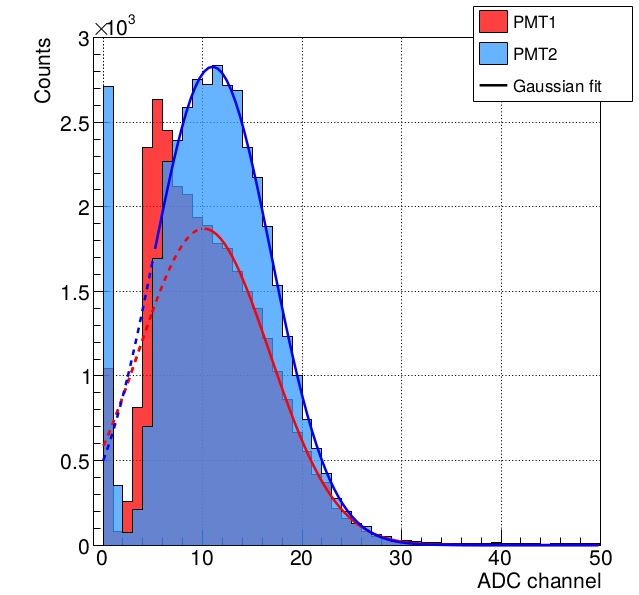
\includegraphics[scale=0.45]{5Prototypes/53FinalPrototypes/531TritiumAveiro/SinglePhotonEnergyDistribution.png}
%\caption{The single-photon energy distribution of both PMTs used in the TRITIUM-Aveiro prototype and their sum \cite{ExperimentalPaperCarlos}.\label{fig:SinglePhotonEnergyDistribution}}
%\end{figure}

%The distributions obtained deviates from Gaussian functions due to the noise in the low energy channels. As DRIM laboratory is not allowed to work with liquid radioactive source such as tritiated water, the first scintillating photons were produced by a $\ce{^{55}Fe}$ radioactive source since the energy of its $\gamma$ emission, $5.9~\keV$, is very close to the energy of tritium electrons. The TRITIUM-Aveiro prototype was coupled to both PMTs using optical grease and the radioactive source was placed inside the PTFE vessel. The prototype was not filled with water for this measurement. The spectra obtained are shown in Figure \ref{fig:55FeMeasurement}. A shift to higher energies is observed in the PMT2 data due to its higher gain and to the closer distance to the radioactive source.

%\begin{figure}[h]
%\centering
%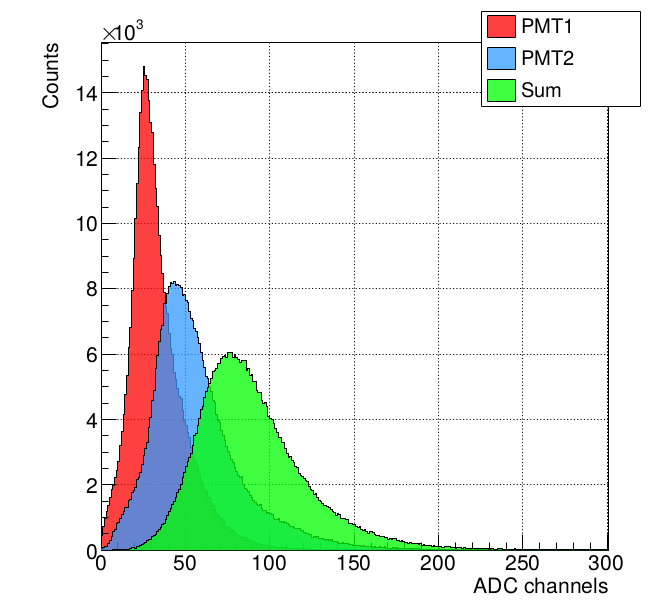
\includegraphics[scale=0.45]{5Prototypes/53FinalPrototypes/531TritiumAveiro/55FeMeasurement.png}
%\caption{Measurement of a $\ce{^{55}Fe}$ radioactive source with the TRITIUM-Aveiro prototype \cite{ExperimentalPaperCarlos}.\label{fig:55FeMeasurement}}
%\end{figure}

First, a measurement with a passive shield was performed in the DRIM laboratory to quantify the attenuation of the background by lead. These measurements, shown in Figure \ref{fig:LeadShieldTest}, were carried out in three different situations. The first, region A, was performed without shielding, the second, region B, with a lead shield of $2.5~\mm$ thickness and the third, region C, with two lead foil layers. As can be seen, in the region A, the average rate of $2.5$ days is $3.5 \cdot{} 10^3$ counts/min. In the region B, a background supression by a factor of 2 was observed, measuring an average rate of $1.6 \cdot{} 10^3$ counts/min. In the region C, an average rate of $0.9 \cdot{} 10^3$ counts/min was obtained, supressing the background by about a factor of 4.

\begin{figure}[h]
\centering
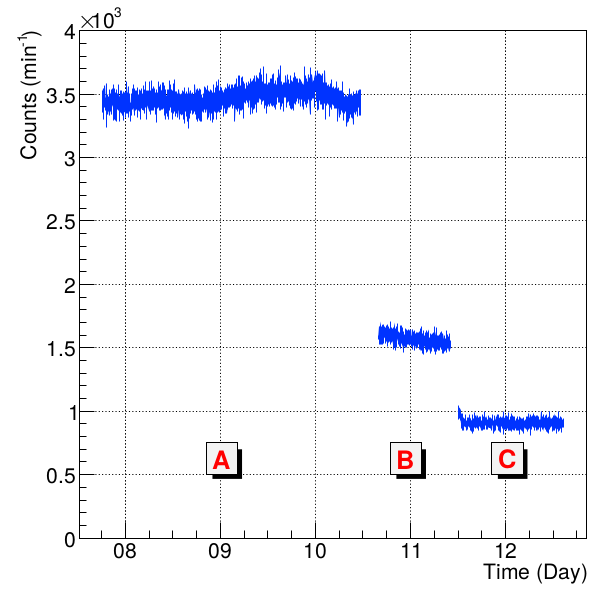
\includegraphics[scale=0.4]{5Prototypes/53FinalPrototypes/531TritiumAveiro/LeadShieldTest.png}
\caption{Measurement of the background with TRITIUM-Aveiro prototype shielded with different layers of lead, A) without shielding, B) with a lead shield of $2.5~\mm$ thickness and C) with two lead shields of $2.5~\mm$ thickness each one \cite{ExperimentalPaperCarlos}.\label{fig:LeadShieldTest}}
\end{figure}

%It has to be taken into account that the case C is the real situation that is present in Arrocampo since, as it has been shown in section \ref{subsec:SetUpActiveShield}, the thickness of the lead shielding ise $5~\mm$.

Then, the prototype was installed in the LARUEX laboratory, at the University of Extremadura, in order to work with a tritiated water. The background of the prototype was measured during 4 days with the prototype filled with pure water and covered with lead bricks of $5~\cm$ thickness. The time adquisition of each measurement was $1$ minut. The data, fitted to a Gaussian function, are shown in Figure \ref{subfig:MeasurementInRealTime}. An average rate of $540$ counts/min with a standard deviation of $22.61$ counts/min was obtained. To calculate the Minimum Detectable Activity (MDA), the detection limit concepts developed by Lloyd A. Currie \cite{CurieLimit} were applied, according to which the minimum net counts with a probability of a false-negative less than a $5\%$, $N_D$, is given by,
\begin{equation}
N_D = 4.65 \cdot{}\sigma_{Nb} + 2.71 = 108~\text{counts/min}
\label{eq:EquationNetCounts}
\end{equation}
which corresponds to a critical level of $Lc = 2.33\cdot{}\sigma_{Nb}=53 ~\text{counts/min}$ (minimum net currents with a probability of a false-positive less than $5\%$).

$L_C$ and $N_D$ refer to the net rate after background subtraction. Therefore, $L_C'$ and $N_D'$, referred to the detector signal (before background subtraction), are $593$ and $648$ counts/min respectively.

\begin{figure}
\centering
    \begin{subfigure}[b]{0.45\textwidth}
    \centering
    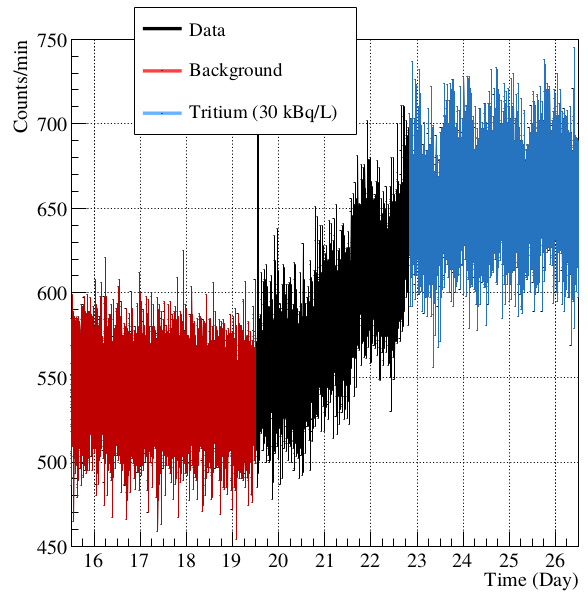
\includegraphics[width=\textwidth]{5Prototypes/53FinalPrototypes/531TritiumAveiro/Tritium_1min.png}  
    \caption{\label{subfig:MeasurementInRealTime}}
    \end{subfigure}
    \hfill
    \begin{subfigure}[b]{0.45\textwidth}
    \centering
    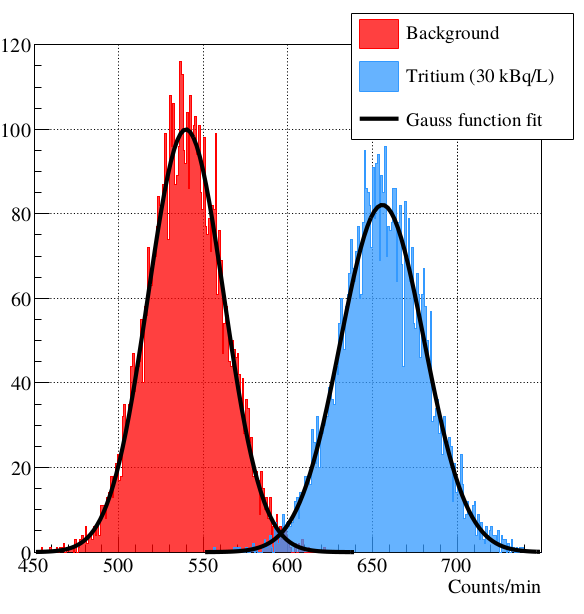
\includegraphics[width=\textwidth]{5Prototypes/53FinalPrototypes/531TritiumAveiro/Tritium_Gaus_1_min.png}  
    \caption{\label{subfig:DistributionofMeasurement}}
    \end{subfigure}
 \caption{Measurements of the background and tritium liquid source (with an activity of $29.8~\kilo\becquerel/\liter$) performed with the TRITIUM-Aveiro prototype and integred during a minute \cite{ExperimentalPaperCarlos}. a) Counts per minut measured as a function of time. b) Distribution of the acquired data.}
 \label{fig:BackgroundTritium1min}
\end{figure}

To find the MDA, tritiated water was slowly added  so that the tritium water activity increased continuously up to reach the $N_D'$ value. An average of $656 \pm 26$ counts/min was obtained, the activity of which was MDA=$29.8~\kilo\becquerel/\liter$, obtained with a Quantulus liquid scintillator system.

The tritium detection efficiency was calculated from the ratio of the net tritium rate measured, $1.93 \pm 0.58$ counts/sec, and the activity of the tritium source used, $29.8~\kilo\becquerel/\liter$. The efficiency obtained is $(6.49 \pm 1.94)\cdot{} 10^{-2}~\frac{cps}{\kilo\becquerel/\liter}$.  and the specific efficiency is
$$S=(1.6 \pm 0.5)\cdot{} 10^{-5}~\frac{cps}{\kilo\becquerel/\liter \cdot{} \cm^{2}}$$ 
Comparing to the specific efficiency obtained with scintillating detectors, Table \ref{tab:PlasticScinTritium}, the specific efficiency of the TRITIUM-Aveiro prototype is close the largest value, obtained by Hofstetter \cite{Hofstetter1, Hofstetter2}, $<2.22~\frac{cps}{\kilo\becquerel/\liter \cdot{} \cm^{2}}$. However this prototype has a lower specific efficiency than TRITIUM-IFIC-1. A possible reason is that the fibers in this prototype are not polished, neither cleaned. 

The efficiency uncertainties obtained for this prototype are larger than those obtained in the first TRITIUM prototypes since the measurement time used is shorted ($1$ minute) than the time used for the previous prototypes (several hours). Because of that, longer measurements are studied to quantify the reduction of the MDA of this prototype, which depends directly on the background uncertainty, equation \ref{eq:EquationNetCounts}. The data for an integrated time of $60$ minutes is shown in Figure \ref{fig:Tritium60min}. The mean value and the uncertainty of the measured background data are $3.186 \cdot{} 10^{4}$ and $228$ counts per hour respectively. Values of $L_C=530$ and $N_D=1043$ counts per hour are obtained from the equation \ref{eq:EquationNetCounts}. Assuming linearity between the measured counts for the background and the tritiated water, the $N_D'$ obtained for this case, $3.872\cdot{}10^4$ counts per hour,  correspons to a MDA of $4.53~\kilo\becquerel/\liter$. A daily oscillation is clearly observed in the Figure \ref{fig:Tritium60min}, indicating that the measurements are affected by external light. This oscillation begins on the $19^{th}$ day, when the water closed circuit pump was installed, so it is likely that a light leak was introduced in the system.

\begin{figure}[h]
\centering
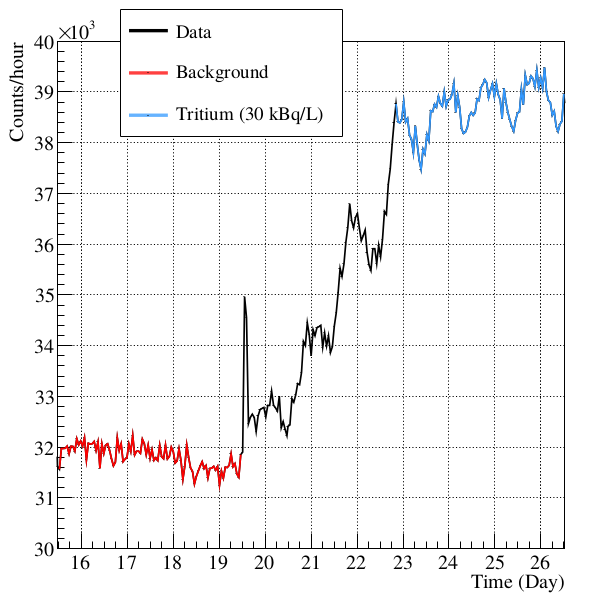
\includegraphics[scale=0.45]{5Prototypes/53FinalPrototypes/531TritiumAveiro/Tritium_60min.png}
\caption{Measurements of the background and tritium liquid source (with an activity of $29.8~\kilo\becquerel/\liter$) performed with the TRITIUM-Aveiro prototype and integrated during one hour \cite{ExperimentalPaperCarlos}.\label{fig:Tritium60min}}
\end{figure}

This prototype was finally installed in the Arrocampo dam to test its functionality and to begin with the tritium level monitoring the measurements of which are reported in section \ref{sec:ResultsArrocampo}.